\documentclass[titlepage]{article}
\usepackage{babel}
\usepackage{amsmath}
\usepackage{amssymb}
\usepackage{amsthm}
\usepackage{multicol} %spalten in seite
\usepackage{graphicx} %bilder einfügen
\usepackage[normalem]{ulem} %durchstreichen
\usepackage{tabto} %tabulator mit \tab
\usepackage{hyperref}
\usepackage{wasysym}
\usepackage{bbm}
\usepackage{tikz}
\usetikzlibrary{shapes.geometric}
\usepackage{bbold}
\usepackage{xcolor}
\usepackage[T1]{fontenc}
\usepackage{mathrsfs}  
\usepackage[utf8]{inputenc}
\usepackage{listings} %quellcode
\pagestyle{plain}
\pagenumbering{arabic}
\renewcommand{\arraystretch}{1.3} %vertikaler abstand von tabellen
\newcommand{\n}{\newline}
\usepackage[left=20mm, right=15mm, top=25mm, bottom=30mm, paper=a4paper]{geometry}
\renewcommand{\contentsname}{Inhaltsverzeichnis}

\newcommand{\K}{\mathbb{K}}
\newcommand{\C}{\mathbb{C}}
\newcommand{\N}{\mathbb{N}}
\newcommand{\Q}{\mathbb{Q}}
\newcommand{\R}{\mathbb{R}}
\newcommand{\1}{\mathbb{1}}
\newcommand{\0}{\mathbb{0}}
\newcommand{\Z}{\mathbb{Z}}

\newcommand{\vecD}[3]{\left(\begin{smallmatrix}#1\\#2\\#3\end{smallmatrix}\right)}
\newcommand{\matrixZ}[4]{\begin{pmatrix}#1&#2\\#3&#4\end{pmatrix}}
\newcommand{\detZ}[4]{\begin{vmatrix}#1&#2\\#3&#4\end{vmatrix}}
\newcommand{\detD}[9]{\begin{vmatrix}#1&#2&#3\\#4&#5&#6\\#7&#8&#9\end{vmatrix}}


\begin{document}
	
	\begin{center}
		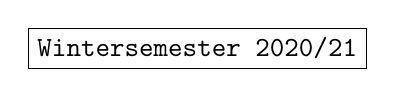
\begin{tikzpicture}
			\draw (0,0) node[draw, rectangle]{\texttt{Wintersemester 2020/21}};
		\end{tikzpicture}
		\hrulefill\\
		\begin{center}
			\LARGE Lineare Algebra - Übung 09 \normalsize\\
		\end{center}
		\hrulefill
		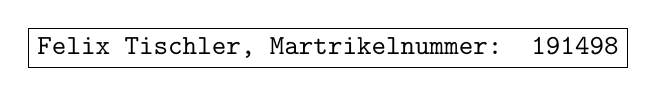
\begin{tikzpicture}
			\draw (0,0) node[draw, rectangle]{\texttt{Felix Tischler, Martrikelnummer: 191498}};
		\end{tikzpicture}
		\date{\today}
	\end{center}
	
	\part*{Hausaufgaben (Abgabe bis 18.01.2021, 14:00 Uhr)}
	\section*{Hausaufgabe 9.1): $Abbildungsmatrizen$ $II$}
		\subsection*{a)}
			Zz. ist, dass wenn $\vecD{x}{y}{z}$ darstellbar als Linearkombination von $\vec{v}_1,\vec{v}_2$ ist, so kann man $\vec{v}_1,\vec{v}_2$ umschreiben und ebenso eine Linearkombination für $\vecD{z}{-x}{y}$ erhalten. Dies ist in Aufgabe (b) implizit gezeigt worden. Es reicht im folgenden $f(\vec{v}_1),f(\vec{v}_2)$ zu betrachten, da sich jeder andere Vektor $f(\vec{a})$ als Linearkombination $\lambda f(\vec{v}_1)+\mu f(\vec{v}_2)$ darstellen lässt. \qed

		\subsection*{b)}
			\begin{align*}
				^B_Bf=(^Bf(\vec{v}_1),\,^Bf(\vec{v}_2))
			\end{align*}
			\begin{align*}
				^Bf(\vec{v}_1)=\,^B\vecD{1}{-1}{0} & &^Bf(\vec{v}_2)=\,^B\vecD{-1}{-1}{-2}
			\end{align*}
			\begin{align*}
				\left(\begin{array}{cc|cc}
					1&1&1&-1\\
					0&-2&-1&-1\\
					1&-1&0&-2
				\end{array}\right)
				\overset{III-I}{\rightsquigarrow}
				\left(\begin{array}{cc|cc}
					1&1&1&-1\\
					0&-2&-1&-1\\
					0&-2&-1&-1
				\end{array}\right)
				\rightsquigarrow
				\left(\begin{array}{cc|cc}
					1&1&1&-1\\
					0&-2&-1&-1
				\end{array}\right)
				\overset{II\cdot-2^{-1}}{\rightsquigarrow}
				\left(\begin{array}{cc|cc}
					1&1&1&-1\\
					0&1&1/2&1/2
				\end{array}\right)	
			\end{align*}
			\begin{align*}
				\overset{I-II}{\rightsquigarrow}
				\left(\begin{array}{cc|cc}
					1&0&1/2&-3/2\\
					0&1&1/2&1/2
				\end{array}\right)
				\Rightarrow
				\,^B_Bf=\matrixZ{1/2}{-3/2}{1/2}{1/2}\qed
			\end{align*}
	\section*{Hausaufgabe 9.2): $Determinanten$ $I$}
	In Hausaufgabe 9.2) und Hausaufgabe 9.3) habe ich die folgenden Regeln und Verfahren wie folgt abgekürzt:
		\begin{itemize}
			\item (S)$\dots$Regel von Sarrus
			\item (L)$\dots$Laplacescher Entwicklungssatz
			\item (B)$\dots$Blockmatrix
			\item (D)$\dots$Dreiecksmatrix
		\end{itemize}
		\subsection*{a)}
		\begin{align*}
			\detZ{3}{2}{-2}{5}\overset{(S)}{=}3\cdot5-(-2)\cdot2=15+4=19
		\end{align*}
		\subsection*{b)}
		\begin{align*}
			\detZ{3}{2}{-9}{-6}\overset{(S)}{=}3\cdot(-6)-(-9)\cdot2=0
		\end{align*}
		\subsection*{c)}
		\begin{align*}
			\detD{1}{-2}{3}{3}{1}{-5}{2}{-3}{3}=1\cdot\underbrace{\detZ{1}{-5}{-3}{3}}_{\overset{(S)}{=}3-15=-12}-3\cdot\underbrace{\detZ{-2}{3}{-3}{3}}_{\overset{(S)}{=}-6+9=3}+2\cdot\underbrace{\detZ{-2}{3}{1}{-5}}_{\overset{(S)}{=}10-3=7}=-12-9+14=-7
		\end{align*}
		\subsection*{d)}
		\begin{align*}
			\detD{\textbf{1}}{-2}{3}{\textbf{3}}{1}{-5}{\textbf{5}}{-3}{1}\overset{(L)}{=}\textbf{1}\cdot\underbrace{\detZ{1}{-5}{-3}{1}}_{\overset{(S)}{=}1-15=-14}-\textbf{3}\cdot\underbrace{\detZ{-2}{3}{-3}{1}}_{\overset{(S)}{=}-2+9=7}+5\cdot\underbrace{\detZ{-2}{3}{1}{-5}}_{\overset{(S)}{=}10-3=7}=-14-21+35=0
		\end{align*}
		\subsection*{e)}
		\begin{align*}
			\begin{vmatrix}
				2&3&1&2\\
				1&1&2&0\\
				0&0&1&-2\\
				0&0&1&2
			\end{vmatrix}
			\overset{(B)}{=}\detZ{2}{3}{1}{1}\cdot\detZ{1}{-2}{1}{2}\overset{(S)}{=}(2-3)\cdot(2+2)=-4
		\end{align*}
		\subsection*{f)}
			\begin{align*}
				\begin{vmatrix}
					1&0&0&0\\
					0&0&1&0\\
					0&0&0&1\\
					0&1&0&0\\
				\end{vmatrix}
				\xrightarrow[\text{\textit{kein Vorzeichenwechsel}}]{II\rightleftarrows IV,\text{ \textit{dann} }IV\rightleftarrows III}
				\begin{vmatrix}
					1&0&0&0\\
					0&1&0&0\\
					0&0&1&0\\
					0&0&0&1\\
				\end{vmatrix}
				\overset{(D)}{=}1
			\end{align*}
	\section*{Hausaufgabe 9.3): $Determinanten$ $II$}
		\subsection*{a)}
		\begin{align*}
			\begin{vmatrix}
				3&-1&7&2\\
				0&0&-1&0\\
				4&\sqrt{2}&37&1\\
				0&2&0&0
			\end{vmatrix}
			\xrightarrow{I-2\cdot III}
			\begin{vmatrix}
				-5&-1-2\sqrt{2}&-67&0\\
				0&0&-1&0\\
				4&\sqrt{2}&37&\textbf{1}\\
				0&2&0&0
			\end{vmatrix}
			\overset{(L)}{=}
			-\textbf{1}\cdot\detD{-5}{-1-2\sqrt{2}}{-67}{0}{0}{-1}{0}{2}{0}\overset{(L)}{=}-1\cdot\left(-5\cdot\underbrace{\detZ{0}{-1}{2}{0}}_{\overset{(S)}{=}2}\right)\overset{(S)}{=}5\cdot2=10
		\end{align*}
		\subsection*{b)}
			\begin{align*}
				\begin{vmatrix}
					1&1&1&1\\
					-1&1&2&3\\
					1&1&4&9\\
					-1&1&8&18
				\end{vmatrix}
				\xrightarrow[III-I]{IV-II}
				\begin{vmatrix}
					1&1&1&1\\
					-1&1&2&3\\
					0&0&3&8\\
					0&0&6&15
				\end{vmatrix}
				\overset{(B)}{=}\underbrace{\detZ{1}{1}{-1}{1}}_{\overset{(S)}{=}2}\cdot\detZ{3}{8}{6}{15}\overset{(S)}{=}2\cdot(3\cdot15-8\cdot6)=90-96=-6
			\end{align*}
		\subsection*{c)}
			\begin{align*}
				\begin{vmatrix}
					1&1&1&1&1&1\\
					2&3&3&3&3&3\\
					3&5&6&6&6&6\\
					1&2&3&4&4&4\\
					1&2&3&4&5&5\\
					1&2&3&4&5&6
				\end{vmatrix}
				\xrightarrow{\substack{II-3\cdot I \\ III-6\cdot I \\ IV-4\cdot I}}
				\begin{vmatrix}
					1&1&1&1&1&1\\
					-1&0&0&0&0&0\\
					-3&-1&0&0&0&0\\
					-3&-2&-1&0&0&0\\
					1&2&3&4&5&5\\
					1&2&3&4&5&6
				\end{vmatrix}
				\xrightarrow[\substack{\text{\textit{kein Vorzeichenwechsel}} \\ \textit{denn es wird 2-mal} \\ \textit{die Zeile vertauscht}}]{I\rightleftarrows IV\text{\textit{, dann }}II\rightleftarrows III}
				\begin{vmatrix}
					-3&-2&-1&0&0&0\\
					-3&-1&0&0&0&0\\
					-1&0&0&0&0&0\\
					1&1&1&1&1&1\\
					1&2&3&4&5&5\\
					1&2&3&4&5&6
				\end{vmatrix}
			\end{align*}
			\begin{align*}
				\begin{vmatrix}
					-3&-2&-1&0&0&0\\
					-3&-1&0&0&0&0\\
					-1&0&0&0&0&0\\
					1&1&1&1&1&1\\
					1&2&3&4&5&5\\
					1&2&3&4&5&6
				\end{vmatrix}
				\overset{(B)}{=}\detD{-3}{-2}{-1}{-3}{-1}{0}{-1}{0}{0}\cdot\underbrace{\detD{1}{1}{1}{4}{5}{5}{4}{5}{6}}_{\left|\begin{smallmatrix}1&1&1\\4&5&5\\4&5&6\end{smallmatrix}\right|\overset{(*)}{\Rightarrow}\left|\begin{smallmatrix}\textbf{1}&1&1\\0&1&1\\0&1&2\end{smallmatrix}\right|}\overset{(L)}{=}-\textbf{1}\cdot\underbrace{\detZ{-3}{-1}{-1}{0}}_{\overset{(S)}{=}-1}\cdot\underbrace{\detZ{1}{1}{1}{2}}_{\overset{(S)}{=}1}=1
			\end{align*}
			(*) II-4$\cdot$I, und III-4$\cdot$I
\end{document}
